\documentclass[serif,xcolor=pdftex,dvipsnames,table,hyperref={bookmarks=false,breaklinks}]{beamer}

%%%%%%%%%%%%%%%%
% Change the macros below to configure the title slides
% for your course.
\newcommand{\coursename}{COMPSCI 589}
\newcommand{\instructor}{Benjamin M. Marlin}
\newcommand{\university}{University of Massachusetts Amherst}
\newcommand{\department}{College of Information and Computer Sciences}
%%%%%%%%%%%%%%%%


\newcommand{\settitlecard}[2]{
  \title[\coursename  Lecture #1] 
    {\coursename \\ Lecture #1: #2}
     \author[\instructor]{\instructor}
     \institute[\university]{
     \department\\
     \university
   }
\date{}
}

\newcommand{\maketitlepage}{
  \begin{frame}
  \titlepage
  \center{
    %If you use the slides unmodified, retain the attribution below
    \tiny{Slides by Benjamin M. Marlin (marlin@cs.umass.edu). \\
    \vspace{-1em}Created with support from National Science Foundation Award\# IIS-1350522. 
    %If you modify the slides, please retain the alternate attribution below
    %\tiny{Based on slides by Benjamin M. Marlin (marlin@cs.umass.edu). \\    
    %\vspace{-1em}Created with support from National Science Foundation Award\# IIS-1350522. 
    }                                              
  }  
  \end{frame}
}

\AtBeginSection[]
{
  \begin{frame}<beamer>{Outline}
    \tableofcontents[currentsection,subsectionstyle=hide]
  \end{frame}
}


\newcommand{\cut}[1]{}

\newcommand{\iconbox}[4]{
  \only<#1-#2>{
    \begin{columns}[T]
      \column{0.5in}
           \includegraphics[width=0.5in]{#3}
       \column{3.7in}
            #4
    \end{columns}
    \medskip
    \medskip
    \medskip
  }
}

\mode<presentation>{
  \usepackage{../beamertheme589theme}
  \setbeamercovered{invisible}
}

\mode<handout>{
  \usepackage{../beamertheme589theme}
  \setbeamercovered{transparent}
}


\usepackage[english]{babel}
\usepackage[latin1]{inputenc}
\usepackage{times}
\usepackage[T1]{fontenc}
\usepackage{amsmath}
\usepackage{amssymb}
\usepackage[noend]{algorithmic}
\usepackage{algorithm}
\usepackage{listings}

\renewcommand\mathfamilydefault{\rmdefault}

\newcommand{\setA}{\mathcal{A}}
\newcommand{\setB}{\mathcal{B}}
\newcommand{\setS}{\mathcal{S}}
\newcommand{\setV}{\mathcal{V}}
\DeclareMathOperator*{\union}{\bigcup}
\DeclareMathOperator*{\intersection}{\bigcap}
\DeclareMathOperator*{\Val}{Val}
\newcommand{\mbf}[1]{{\mathbf{#1}}}
\DeclareMathOperator*{\argmax}{arg\,max}
\DeclareMathOperator*{\argmin}{arg\,min}
\DeclareMathOperator*{\sign}{sign}
\newcommand{\deriv}[2]{\frac{\partial{#1}}{\partial{#2}}}


\settitlecard{16}{K-Means Clustering}

\begin{document}

\maketitlepage

\section{Review}
\subsection{Foo}


\begin{frame}[t]{The Clustering Task}
\begin{block}{Definition: The Clustering Task}
Given a collection of data cases $\mbf{x}_i\in\mathbb{R}^D$, partition the 
data cases into groups such that the data cases within each partition are
more similar to each other than they are to data cases in other partitions.
\end{block}
\end{frame}
 
 
\begin{frame}[t]{Defining a Clustering}
 
\begin{itemize}
\item Suppose we have $N$ data cases $\mathcal{D}=\{\mbf{x}_i\}_{i=1:N}$.
 
\item A clustering of the $N$ cases into $K$ clusters is a partitioning 
 of $\mathcal{D}$ into $K$ mutually disjoint subsets 
 $\mathcal{C}=\{C_1,...,C_K\}$ such that 
 $C_1 \cup ... \cup C_K = \mathcal{D}$.
 
\end{itemize} 
\end{frame}

\begin{frame}[t]{The Hierarchical Agglomerative Clustering Algorithm}
\center
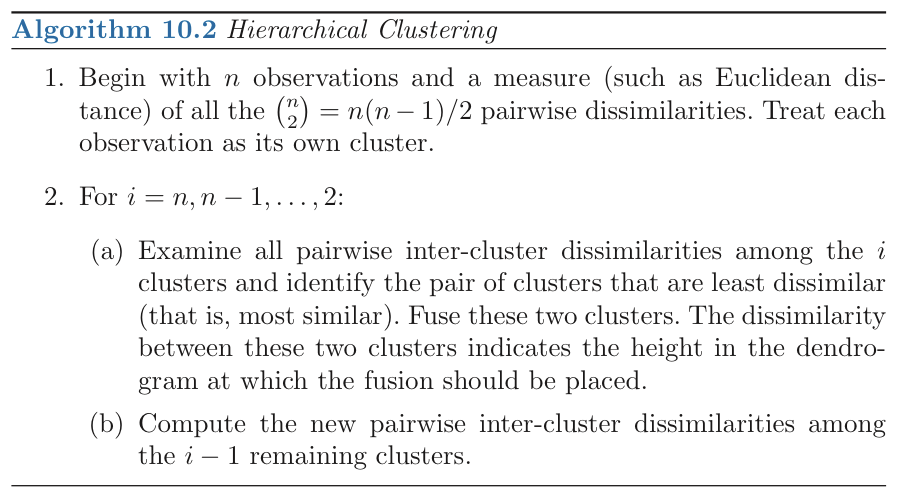
\includegraphics[width=4in]{../Figures/hac_algorithm.png}
\end{frame}


\section{K-Means}
\subsection{Foo}

\begin{frame}[t]{The K-Means Algorithm}
 
\begin{itemize}
\item The K-Means algorithm is an iterative optimization 
algorithm for clustering that alternates between two steps.

\pause \item The algorithm maintains a set of $K$ cluster centroids  or 
prototypes $\mu_k$ that represent the average (mean) feature vector of the data 
cases in each cluster.

\pause\item In the first step, the distance between each data case and each 
prototype is computed, and each data case is assigned to the nearest prototype.

\pause\item In the second step, the prototypes are updated to the mean of the 
data cases assigned to them.

\end{itemize} 
\end{frame}

\begin{frame}[t]{The K-Means Algorithm}

\center
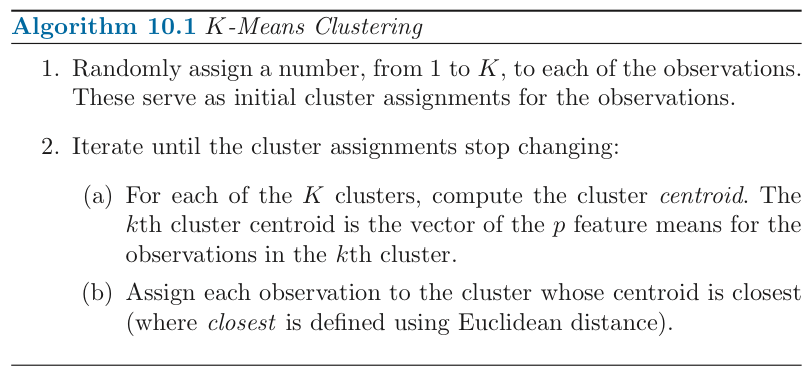
\includegraphics[width=4in]{../Figures/kmeans-algorithm.png}

\end{frame}

\begin{frame}[t]{The K-Means Algorithm}

Suppose we let $z_i$ indicate which cluster $\mbf{x}_i$ belongs to and 
$\mu_k\in \mathbb{R}^D$ be the cluster centroid/prototype for cluster $k$.
The two main steps of the algorithm can then be expressed as follows:

\begin{enumerate}
\item $\displaystyle z_i =\arg\min_k ||\mu_k-\mbf{x}_i||_2^2$

\item $\displaystyle \mu_k = \frac{\sum_{i=1}^N [z_i=k]\mbf{x}_i}{\sum_{i=1}^N 
[z_i=k]}$

\end{enumerate}

\end{frame}

\begin{frame}[t]{The K-Means Objective}

\begin{itemize}
\item The K-Means algorithm attempts to minimize the sum of the within-cluster
variation over all clusters (also called the within-cluster sum of squares):

$$\mathcal{C}^* = \arg\min_{\mathcal{C}} 
\sum_{k=1}^K\frac{1}{|C_k|}\sum_{\mbf{x}_i,\mbf{x}_j\in C_k} 
||\mbf{x}_i-\mbf{x}_j||_2^2$$

\pause\item Note that this objective function has many, many local optima in 
general, each corresponding to a different clustering of the data. 

\pause\item K-Means produces a non-increasing sequence of objective function 
values and is guaranteed to converge to some local optima. Finding the global
optimum is not computationally tractable.


\end{itemize} 

\end{frame}


\begin{frame}[t]{Initialization}

\begin{itemize}
\item Because K-Means finds a local optimum, it can be highly sensitive to 
initialization.

\pause\item It is common to perform multiple random re-starts of the algorithm
and take the clustering with the minimal total variation.

\pause\item Common initializations include setting the initial 
centers to be randomly selected data cases, setting the initial partition to
a random partition, and selecting centers using a ``furthest first''-style 
heuristic (more formally known as K-Means++).

\pause\item It often helps to initially to run with $K\log(K)$ 
clusters, then merge clusters to get down to $K$ and run the algorithm
from that initialization.

\end{itemize} 

\end{frame}

\begin{frame}[t]{Issues}

\begin{itemize}
\item Only works with Euclidean distance. An alternate version based on 
Manhattan distance exists and is called the K-medians algorithm.

\pause\item Pre-processing like re-scaling/normalizing features can
completely change the results.

\pause\item We need some way to determine the ``right'' number of clusters to 
focus on. We want to cluster on salient differences between data cases, not 
noise.

\pause \item The run time is $O(NKT)$ where $T$ is the number of iterations to
convergence of the total variation. $T$ is often small (like 20), but examples 
can be constructed that require an exponential number of steps to converge. 

\pause \item Results in a hard assignment of data cases to clusters, which may 
be a 
problem if there are outliers.

\end{itemize}
\end{frame}


\end{document}
